\documentclass[11pt]{article}
\usepackage{fullpage}
\usepackage{graphicx}
\usepackage{url}
\usepackage{ulem}

\usepackage{clrscode}
\usepackage{amsmath}
\usepackage{amssymb}
\usepackage{url}
\usepackage{graphicx}


\title{CS140 - Assignment 4\\\small{Due: Sunday, February 18 @ 10pm}}
\author{}
\date{}


\begin{document}
\maketitle

\vspace{-.5in}


\begin{center}
% \includegraphics[scale=0.6]{figures/math.jpg}
% \footnotesize{http://www.smbc-comics.com/index.php?db=comics\&id=1872}
\end{center}

\noindent You may (and are encouraged) to work with a partner on this assignment. If you're looking for a partner, post on slack (or email me).  Please do this sooner than later!\\

\begin{enumerate}

\setcounter{enumi}{-1}

\item \emph{Optional:} We're about a third of the way through the course and I wanted to checkin and see how things are going.  I've gotten some feedback the group assignments, but I'd also love to get individual feedback on things.  If you want (it's anonymous), take 5 minutes and let me know how things are going:

\url{https://forms.gle/tfjwU7igYkNxy1gR8}

\item \textbf{[12 points]} In a binary search tree, we might also keep track of the total number of nodes in that subtree (including the node itself).

\begin{enumerate}

\item \textbf{[5 points]} Assuming we store this value (e.g. $x.size$) write pseudocode for a function \textsc{BSTKeyLessThan($T,k$)} that takes a tree $T$ and a number $k$ and returns the number of values in the tree $T$ that are less than $k$.  For example, if the tree had the number 1 through 9 in it, then  \textsc{BSTKeyLessThan($T,5$)} should return 4.  You will be graded on how efficient your algorithm is and how effectively you utilize the tree structure.  For example, traversing the entire tree and counting all of the values would not get very many points.

\begin{codebox}
\Procname{$\proc{BSTKeyLessThan}(T, k)$}
\li \If $T \leftarrow NULL$
\li     \space \space \space \space \Return $0$
    \End
    
\li \If $T < k$
% \li \If $T.key < k$
\li  \Return $1 + \proc{Left(T)}.size + \proc{BSTKeyLessThan}(\proc{Right(T)}, k)$
\li \Else
\li     \Return $\proc{BSTKeyLessThan}(\proc{Left(T)}, k)$
    \End
\end{codebox}


% \begin{codebox}
% 		\Procname{$\proc{Mystery1}(A)$}
% 		\li $x \gets -\infty$
% 		\li \For $i \gets 1$ \To $\id{length}[A]$
% 		\li	\If $A[i] > x$
% 		\li		$x \gets A[i]$
% 			\End
% 		 \End
% 		\li \Return $x$
% 	       \end{codebox}

% 		\begin{codebox}
% 		\Procname{$\proc{Mystery2}(A)$}
% 		\li \For $i \gets 1$ \To $\lfloor\id{length}(A)/2\rfloor$
% 		\li 	 swap $A[i]$ and $A[\id{length}(A) - (i-1)]$
% 			\End
% \end{codebox}


\item \textbf{[2 points]}  What is the best-case and worst-case running time of your algorithm?  State your run-time with respect to either $n$ the number of nodes or $h$ the height of the tree, whichever is more precise.

The worst case performance occurs with a severely unbalanced BST, specifically a right-leaning twig. The entire tree must be traversed down to the terminal null node to complete the operation. This situation typically unfolds when the tree's structure is sorted, with the search key $k$ located at the end of the tree $(O(n)$. Take the scenario where our root node contains a small value like 1 and our right-leaning twig runs till 100, and our $k=101$, we would have to traverse the entire tree resulting in an $(O(n)$ time complexity.

The best -case scenario would be a BST is  either left-leaning with everything smaller than k  or right leaning has everything greater  than K. In both of the case, h is just equal to n because they are left/right leaning. In the first case, when we compare the root node with the k, and since the root node is less than the k, so we know everything else on the left side would be less than the k, and we only add the size of the left tree and because it's left learning  so the right tree is empty so we only make one comparison.  The running time would be O(1). In the second case, when we compare the root node with the k, and since the root node is greater than the k, so we know everything else on the right side would be greater than the k as well so we don't have anything less than k on the right side, and  because it's right learning the left tree is empty so we only make one comparison. The running time would be O(1).
\item \textbf{[5 points]}  Describe an algorithm \textsc{Median($T$)} that finds the median element in a binary search tree.  You don't have to write pseudocode, but if you don't, make sure that you state your algorithm precisely.  \emph{Hint:} you likely will need some sort of helper function.  State your run-time with respect to either $n$ the number of nodes or $h$ the height of the tree, whichever is more precise.
 
Base case: 
We call the size of the BST, and we divide the size by two, which is  the index of median. 1. Once the index of the median hits zero, we return the value of current node.

Recursive case: 
1.the index of the median is  not zero  =>Then we call size of left tree: 
2. if the size of the left tree is less than the median position then we need to go to the right. The median index minus the size of the left tree and 1 for root node. Then we get the new index for the median to look at the first node in the right tree.   
3. if the size of the left tree is greater than the median position then we go to the first node on the left tree.
recursively do the comparison of the left size of the tree to the new median index, until the index is zero.
The runtime is O(logn).


\end{enumerate}
  
\item \textbf{[26 points]} Stacks and queues

Assume you're given an implementation of a stack that supports {\tt push} and {\tt pop} in $O(1)$ time.  Now you'd like to implement a queue using these stacks.

\begin{enumerate}
\item {[10 points]} Explain how you can efficiently implement a queue using two of these stacks.  (``Efficiently'' means in a way that allows you to do the next part of the problem.)

\textbf{Answer}:

Stack A serves as the destination for all incoming elements during enqueue operations, regardless of Stack B's current contents. Stack B is designated for dequeue operations.

Upon the call of the call of dequeue operations, a preliminary check of Stack B's occupancy is conducted. If found vacant, a transferal of all items from Stack A to Stack B happens by popping items from stack A and pushing them onto stack B, effectively rendering Stack A empty and reordering Stack B into a queue-like configuration that honors the first-in-first-out (FIFO) principle. This reordering is attained by positioning the elements initially at the bottom of Stack A to the top of Stack B.

Following the transfer, or if Stack B was initially non-empty, the dequeue operation is put into effect by executing a pop on Stack B, which eliminates and returns the topmost element (what is called {\tt popleft}). In the event that a dequeue is called while both stacks are empty, an exception is raised to signify the absence of elements in both stacks.

\item {[8 points]} Prove that the amortized cost of each {\tt enqueue} and {\tt dequeue} operation  is $O(1)$ for your stack-based queue by using the the aggregate amortized analysis technique.

\textbf{Answer}:

To assess the amortized cost, we examine the operations over a sequence of \(n\) activities. By analyzing the total cost and dividing by the number of operations, we can calculate the amortized cost per operation.

Consider the sequence of operations:
\[
\begin{array}{ccccccccc}
e & e & d & d & e & e & e & d & d \\
\end{array}
\]
and let's analyze the operations needed to remove element 2.

Initially, after two `enqueue` operations, stack A contains [1, 2], requiring one operation per addition. Upon the first `dequeue`, stack B, being empty, necessitates transferring elements from A, involving two actions: one for popping from A and another for pushing onto B, resulting in stack B as [2, 1].

The `dequeue` operation then demands the removal of the top element from B, reducing B to [2] after popping 1, and a subsequent `dequeue` clears B by popping 2. This final removal counts as a single operation.

Summing these, the process to eliminate the second element involves $1+2+1=4$ operations. Generalizing this to $n$ elements, we find the procedure demands $O(4n)$ operations. However, for amortized analysis, dividing this total by $n$ reveals that each `enqueue` and `dequeue` operation incurs an amortized cost of $O(1)$.

\item {[8 points]} Prove the same amortized constant time using the accounting method for amortized analysis.

\textbf{Answer}:

To determine the bank deposit required to manage the operations of enqueueing and dequeueing, we need to allocate specific costs to these operations and tally them. Based on our initial estimate from the amortized analysis conducted in part b, it appears that a total of 4 monetary units, say Kenyan Shilling (KSh), are necessary to accommodate the expenses of both enqueueing and dequeueing actions.

The enqueue operation incurs a charge of 1 KSh, pushing an element onto stack A. Conversely, the dequeue operation is more costly, amounting to 3 KShs: this includes 1 KSh for popping an element from stack A, another KSh to transfer (push) the element to stack B, and a final KSh for the eventual removal (pop) of this element from stack B.

Consequently, the aggregate cost amounts to 4 KShs, reinforcing the conclusion drawn through the accounting method that the amortized cost per operation is \(O(1)\).
\end{enumerate} 

\item \textbf{[10 points]} Your friend (who hasn't taken algorithms) needs your help.  They think that they have found another method for sorting data that is $O(n \log n)$ but needs your help proving it.  Given an array of $n$ numbers, $A$, the idea is as follows:

\begin{itemize}
\item Call \texttt{BuildHeap} (the $O(n)$ version that creates a \emph{max}-heap) on the array to get a heap.
\item Then, you swap the element at the root with the element at location $n$ and decrement the value of $n$
\item You then call \texttt{BuildHeap} but with a heap size reduced by one (so that it will ignore everything after the most recently copied element).
\item You repeat this process $n$ times.
\end{itemize}

\begin{enumerate}
\item Is the algorithm correct (i.e. will is always sort an array)?  Clearly and succinctly explain your answer.

  Yes. we have a max heap and we keep swapping the max with the min. The max is at the nth spot which is the sort position and we repeat it for n times until the data is sorted.
        
\item What is the run-time of this algorithm?

The run time would be O($n^2$) because we call n times of  buildheap which is O(n). So the total running time would be O($n^2$) . 
\item Is there a way we could modify \texttt{BuildHeap} to create a new function \texttt{HeapFix} and call this in the third step instead of a full call to \texttt{BuildHeap} that would result in a better run-time?  If no, explain why not.  If yes, then briefly explain the algorithm (no need for pseudocode).

\end{enumerate}
we should use heapify instead of build heap because heapify is O(logn) and build heap is O(n). If we do it for n times it would be O(nlogn) with heapify.  After we call buildheap, we already have a heap and we don't need to build a heap again on a recursive call. if we call heapify, we can get a sorted heap.  
\item \textbf{[6 points]} Binomial heaps

\begin{enumerate}

\item Insert the following numbers into a min-ordered (i.e., smaller values have higher priority, like in the notes) binomial heap: \texttt{7, 1, 3, 8, 2, 4, 10, 9}.  Insert the values in that order. Show what the heap looks like after inserting the 2 as well as the final tree after inserting 9.  You can visualize the heaps however you want as long as we can understand it.

    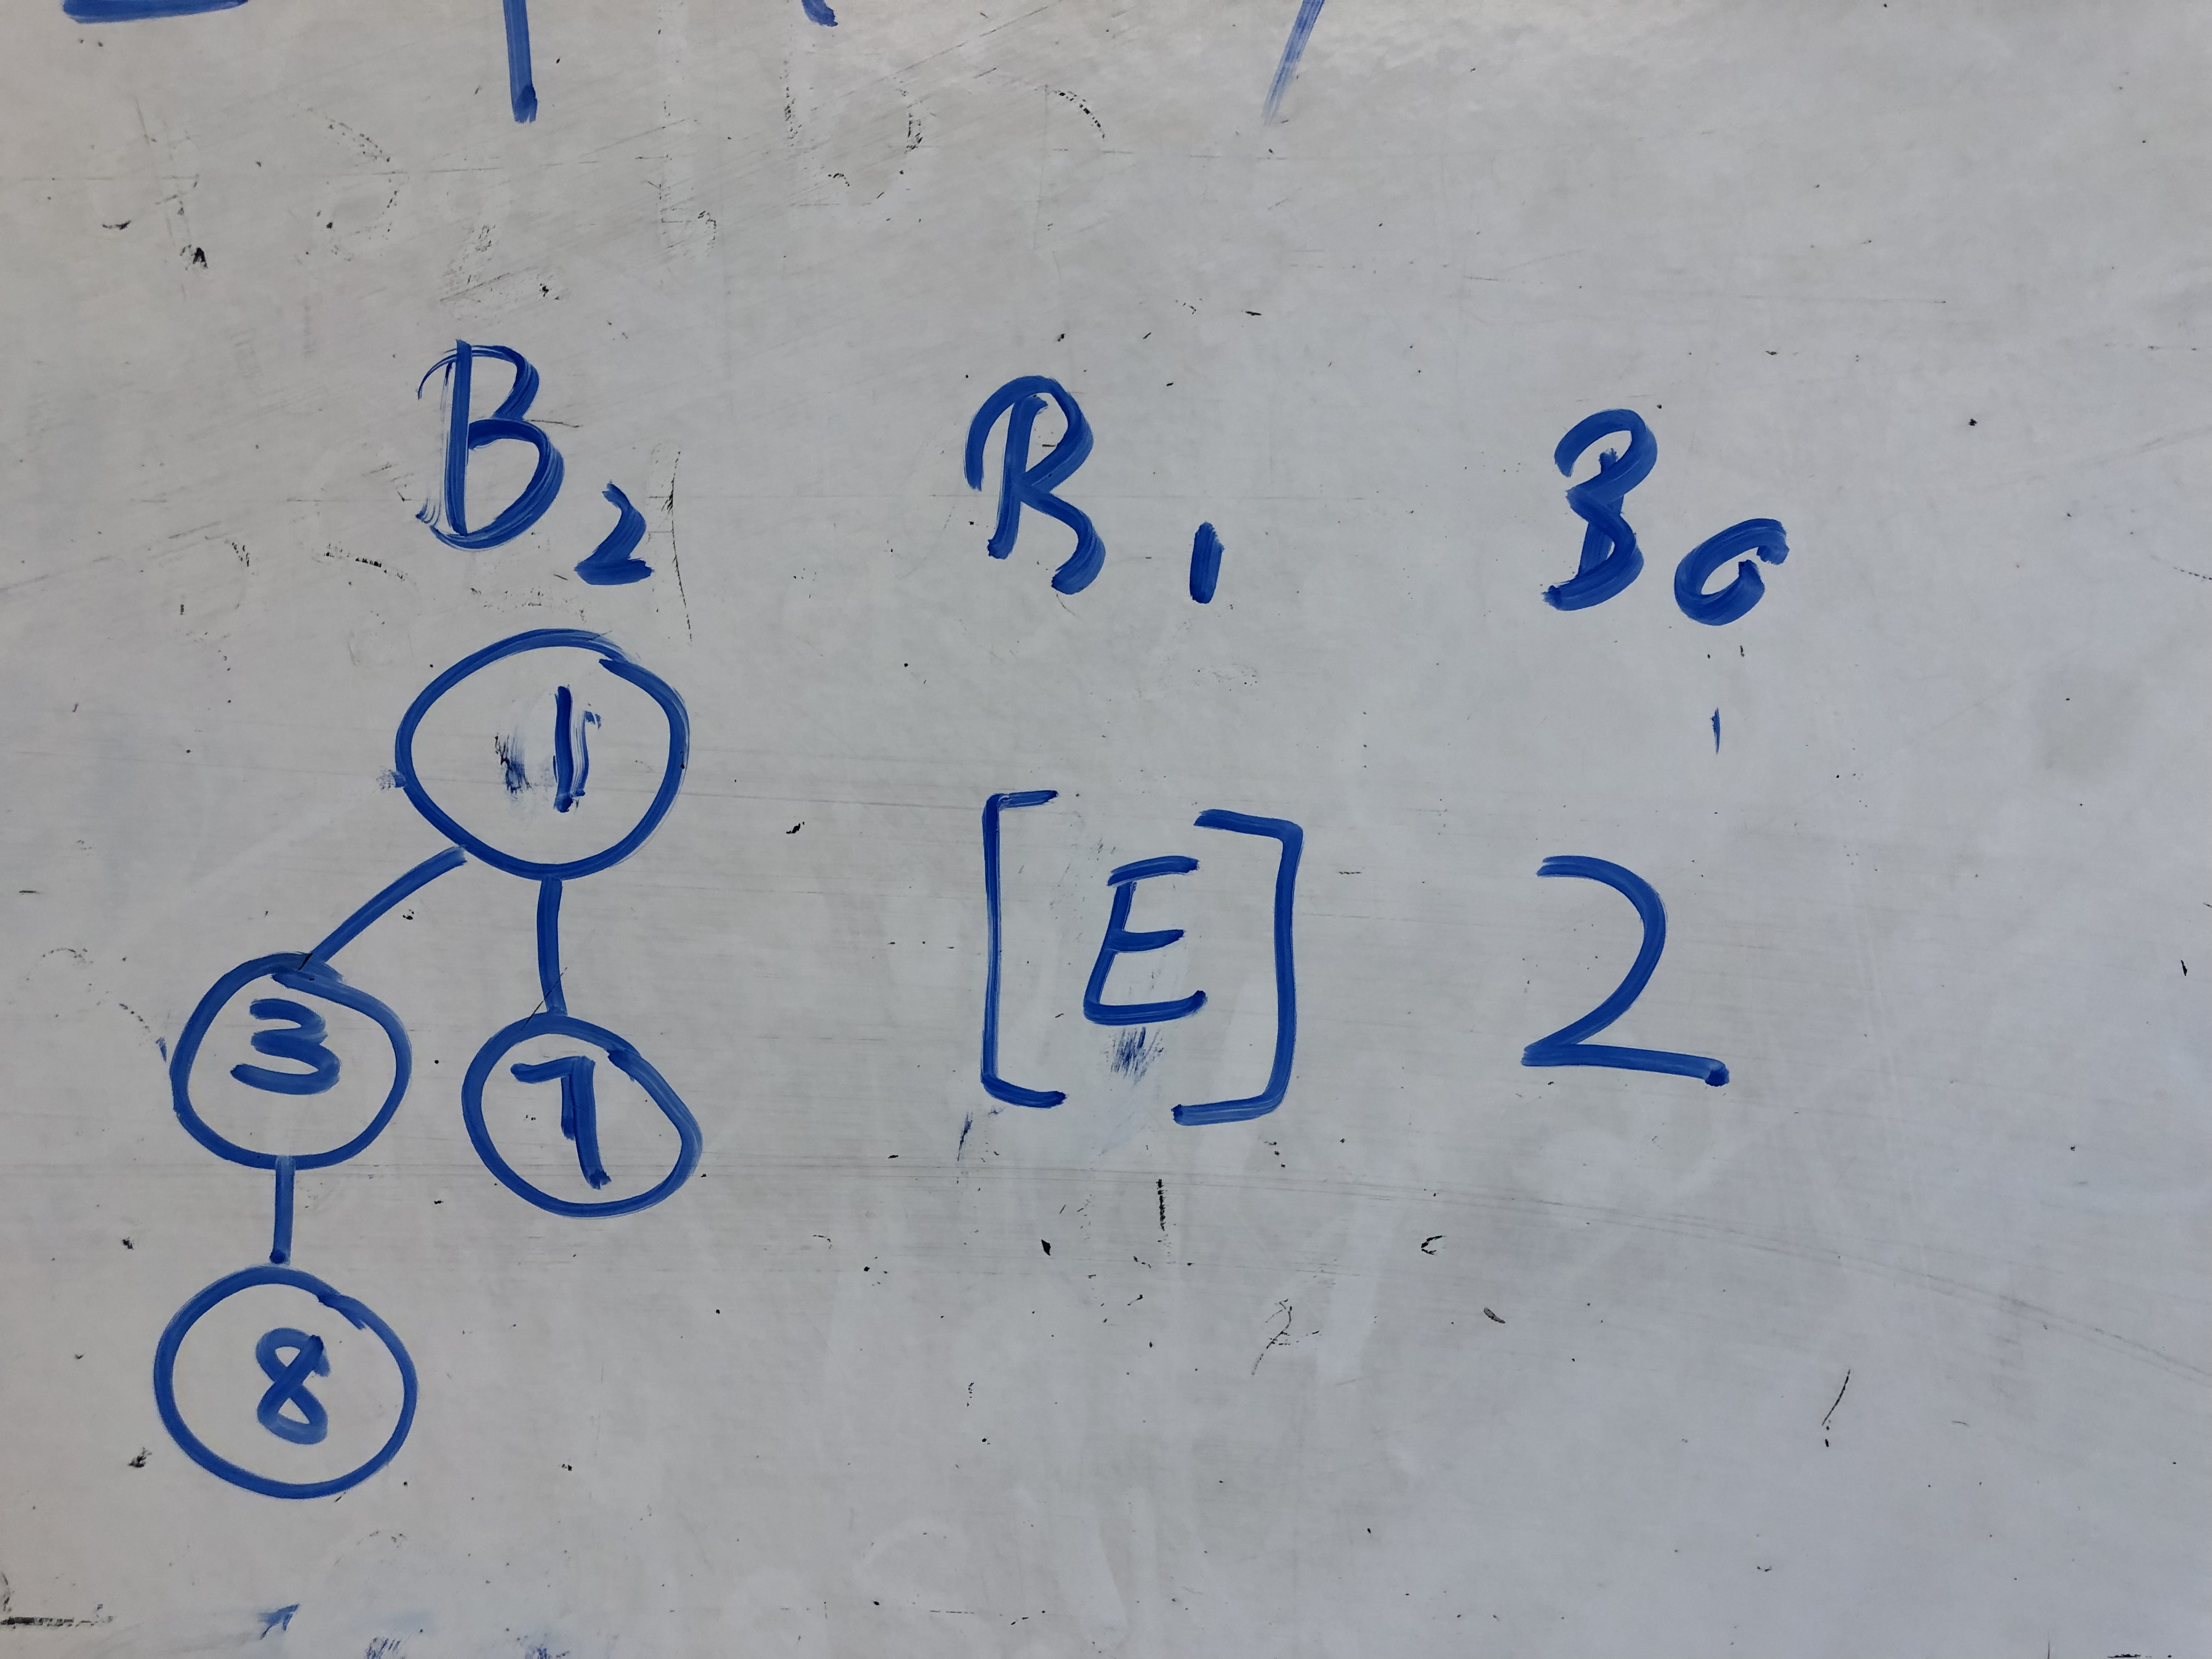
\includegraphics[width=0.5\linewidth]{WechatIMG36.jpeg}

    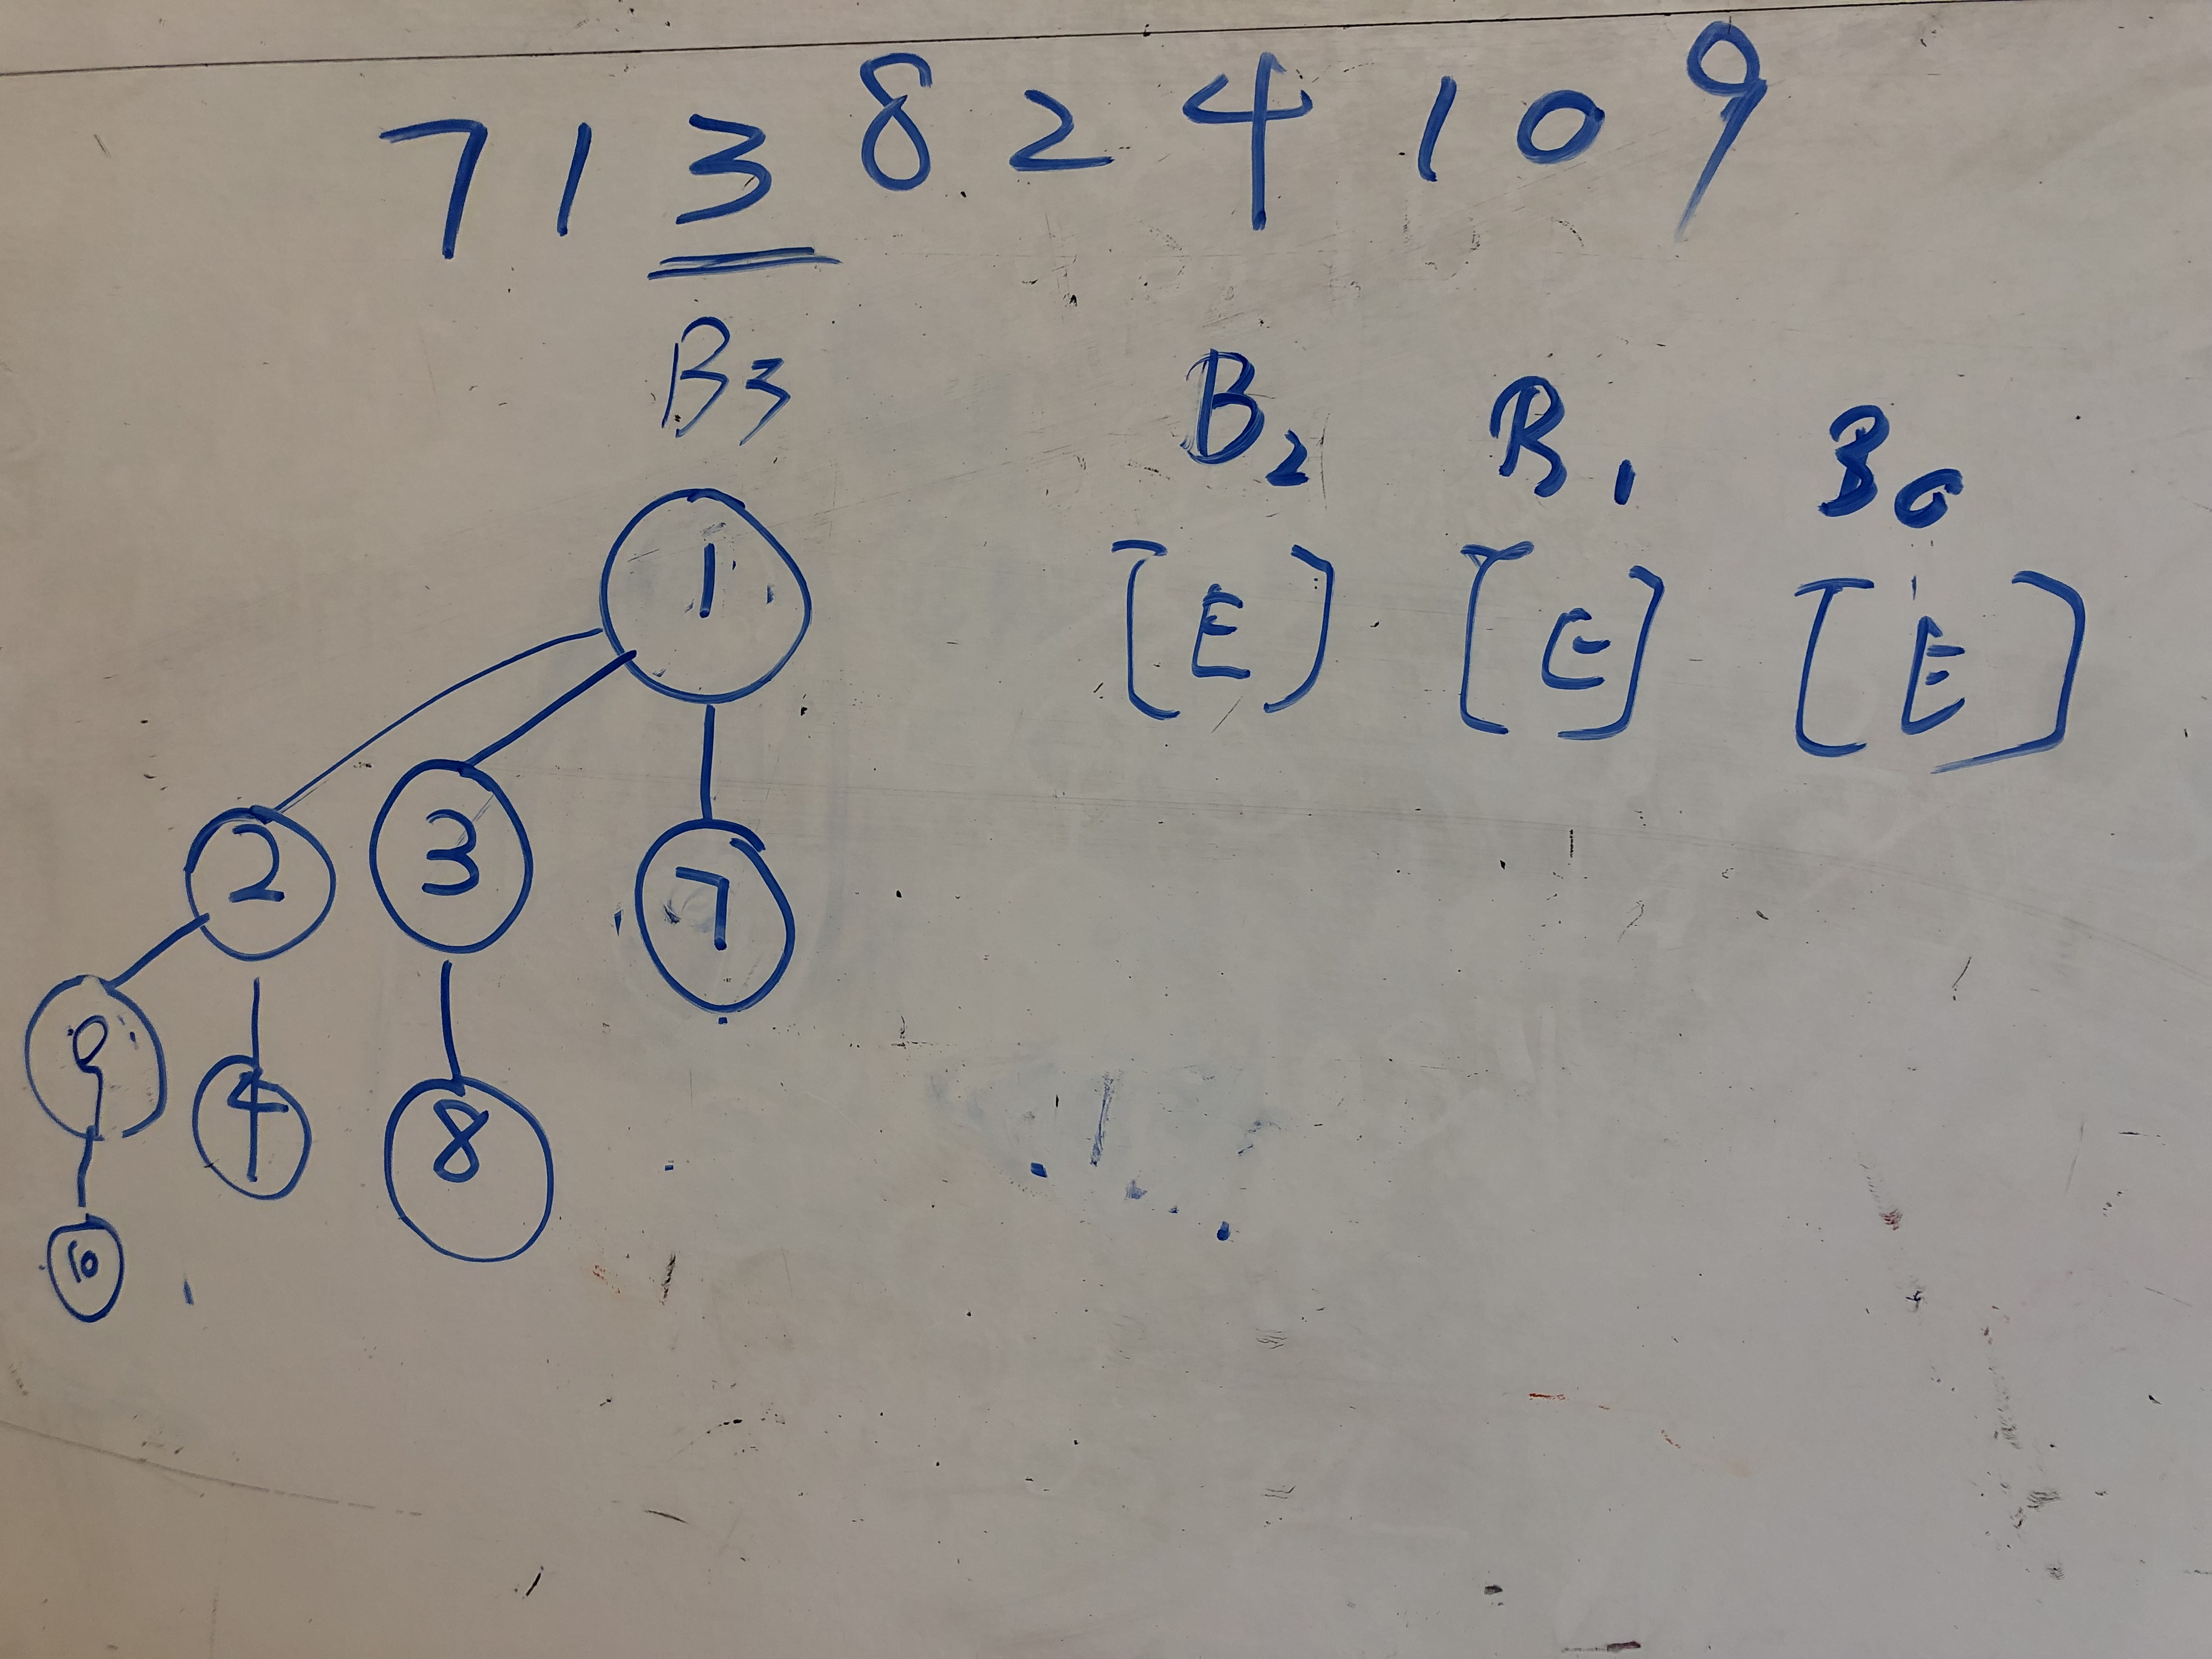
\includegraphics[width=0.5\linewidth]{WechatIMG35.jpeg}

\item A binomial heap is a collection of heap-ordered binomial trees.  If we count ``empty'' trees, the number of binomial trees that makes up the heap only increases occasionally.  For example, if you have a binomial heap with one item and you insert a second item, you go from one binomial tree to two binomial trees (one empty and one with two things in it).  If you insert elements into a binomial heap one at a time, for what values of $n$ will the number of binomial trees in the heap increase (including ``empty'' trees)?

\textbf{Answer}:
The number of binomial number of trees will increase each time you reach to power of 2, which is just $2^k$.

\end{enumerate}
 
\end{enumerate}
\end{document}
